%Chapter 1

\renewcommand{\thechapter}{1}

\chapter{Introduction}

\section{Extragalactic Astronomy: The beginning}
Nebulae, which stand for clouds in Latin, have been an integral part of astronomy since the Middle Ages and were one of the main driving forces behind extragalactic hypotheses. Their first known record dates back to 150 AD, who recorded five objects in the sky as ``nebulous'' in his books VII-VIII  of \textit{Almagest}. Abd al-Rahman al-Sufi noted a ``little cloud'' during 964 AD in his work \textit{Book of fixed Stars}, which we now know as the Andromeda Galaxy. On July 4th, 1054, Chinese and Persian astronomers have recorded the supernova event of the Crab nebula.

With the advent of refracting telescopes, mainly built based on the designs developed by Hans Lippershey in the early 17th century, Orion nebula has been detected and studied in detail by French and Swiss astronomers. Several more nebulae have been cataloged by the middle of the 18th century. In 1715, Edmund Halley published a list of six, Jean-Philippe de Cheseaux twenty with eight newer ones in 1745, Nicolas Louis de Lacaille 42 between 1751-1753. Later in 1781, Charles Messier compiled a list of 103, which are now called Messier objects, including the famous M87.

The number of known objects substantially improved with the works of William Herschel and his sister Caroline who published catalogs with more than a thousand nebulae during the 1780s. However, it was unclear at the time whether some of these objects were located outside the Milky Way. Based on the work of \cite{wright1750original}, who explained the Milky Way as a humungous spinning disk with several layers of stars, \cite{kant1797allgemeine} hypothesized that some nebulae with a fuzzy spiral shape might be independent Milky Ways themselves and termed them ``island universes''. He also suggested the others were thin gas and dust clouds within the Milky Way, collapsed into a spinning disk forming stars and planets, commonly called the nebular hypothesis--both commonly interpreting nebulae as collections of stars.  \cite{10.2307/106755} later noted a reddish region in the central regions of Andromeda, which did not appear anything like a star or known gaseous nebulae, advancing Kant's extragalactic hypothesis. These results resulted in an intense debate in the community. Many astronomers sided with Laplace, who maintained the nebular hypothesis view for spiral nebulae, while a few believed in the extragalactic origin. 

\citet{huggins1864xiii} noted that the spectra of Andromeda resemble a continuum overlaid with absorption lines and concluded that they were stellar in nature. \citet{fath1909spectra} found similar spectra in a few more nebulae. Interestingly some emission lines from one nebula, NGC 1068, were found to have a width of  $\sim$3000 km/s, similar to the lines found in nearby gaseous nebulae, supporting both the hypotheses. Later \citet{slipher1913radial} noted that the lines from Andromeda display a redshift higher than the escape speed of Milky Way, thereby indicating an extragalactic origin. These conflicting views sparked the ``Great Debate'' in astronomy \citep{1921BuNRC...2..171S} between Harlow Shapley and Heber Curtis in April 1920, each favoring the nebular and extragalactic views, respectively, based on different arguments. For example, Shapley argued that the energy output of the nova observed in Andromeda \citep{1888MNRAS..48..108B} would be physically impossible to explain if it were an external galaxy. Conversely, Curtis showed that the nova events in Andromeda outnumbered those in Milky Way and questioned why the events must be disproportionately large in a specific region of the Milky Way if Andromeda were to be a part of it.

Later, \citet{opik1922estimate}  estimated the distance of Andromeda to be about 450 kpc (which is half the actual value), placing it well outside our Galaxy. The debate was finally settled in the late 1920s by \citet{hubble1929relation} who used Cephid variables to confirm Andromeda's extragalactic origin. Cephids are stars with a cycle of brightness whose frequency correlates with their luminosity, allowing us to determine their distance. 

\section{Active Galactic Nuclei: A new paradigm}
Although Hubble's work validated the presence of extragalactic objects, the nature of the bright emission lines from centers some galaxies, however,  remained unknown for a decade or two.  \citet{seyfert1943nuclear} obtained the spectra of six galaxies and found that they show high-excitation emission lines superimposed on a solar-like continuum with widths reaching up to 8500 km/s. These types of galaxies are now called as \textit{Seyfert Galaxies}.  \citet{woltjer1960magnetostatic} noted that parsec scale emission from these galaxies requires a mass of $\sim 10^8$ solar masses ($M_\odot$). \citet{fowler1963star} made an important advance by suggesting that the centers of these galaxies host a massive star; they would emit by accreting dust from the surroundings. A year later, another idea emerged, which assumed that the central object is a black hole rather than a massive star \citep{salpeter1964accretion,zel1964estimating}. Such galaxies, whose bright centers are powered by accretion onto a black hole, are what we now call Active Galactic Nuclei (AGN). AGN are the most luminous and steady sources of luminosity in the universe. They have a broad spectrum covering 20 orders of magnitude in frequency, and their luminosity ranges from $10^{40}-10^{49}$ ergs s$^{-1}$ and are one of the most actively studied classes of objects in astronomy.

\subsection{Radio Astronomy}
Radio astronomy also provided essential contributions to our understanding of AGN. Its history dates back to the early 1930s. In 1932, Karl Guthe Jansky, an engineer at Bell Labs, noted that a radio signal peaked with a period of 24hrs and suspected that they were radio waves from the Sun. Upon gathering more data, he found that the signal repeated with the frequency of a Sidereal day: the time it takes for distant stars to rotate once in our field of view. These findings eventually led Jansky to conclude that the signal came from the central regions of our galaxy \citep{jansky1932directional}, and it marked the first serendipitous discovery of an astronomical radio source and the birth of radio astronomy. He was honored for his seminal contributions to this field by naming the units of flux as Jansky (Jy) after his name.

Inspired by this discovery, Grote Reber, an amateur radio engineer, built a parabolic radio telescope in his backyard with a 9m diameter. He mapped the emission from the galactic center at 160 MHz and not only confirmed Jansky's discovery \citep{reber1940cosmic} but also showed that the emission exhibits a non-thermal spectrum. Although World War II intervened during this period and hindered research in astronomy, it led to advances in radar technology and, consequently, in radio astronomy. 

Martin Ryle and Antony Hewish developed Earth-rotation aperture synthesis techniques in the 1950s, allowing emulation of a large aperture-telescope using a network of several spatially-separated smaller telescopes called baselines. With the arrival of efficient computing machines capable of performing the required inverse Fourier transforms, it was possible to build radio telescopes with one mile and later with 5 km apertures. These telescopes 
%The brightness temperatures of some sources are greater than $10^6 K$ and indicate a non-thermal origin \citep[e.g.,][]{bolton1948variable}. 
%\citet{1950AuSRA...3..234S} located a bright radio source that coincided with the location of M87, which we now identify as a nearby AGN. Later, \citet{1954ApJ...119..215B} identified extended optical emission from M87.
were used to conduct the 3C and 3CR sky-surveys at 159 MHz and 178 MHz, respectively, detecting several hundreds of radio sources \citep{1959MmRAS..68...37E,10.1093/mnras/125.1.75} including well-known sources like 3C 48 and 3C 273. While some had extremely faint star-like optical detections showing emission lines matching with no known element on earth at that time \citep{1963ApJ...138...30M}, the low resolution of these surveys precluded accurate identification of optical counterparts for many of them. Their optical variability ruled out a normal galaxy-like origin, and their extreme brightnesses prevented a stellar interpretation, leading astronomers to call such sources as \textit{quasi-stellar (star-like) sources}, shortened to \textit{quasar} \citep{chiu1964gravitational}. 

\subsection{Discovery of Quasars}
A few years later, measurements of 3C 273 based on lunar-occultation technique allowed  \citet{schmidt19633c} to identify its optical counterpart with a magnitude of 13, again showing unknown lines; it also contained a structure he referred to as ``a faint wisp or jet.'' They both lay close to the radio positions of two bright components in 3C 273. The optical spectrum of  3C 273 exhibited a complex continuum with broad emission lines \citep{oke1963absolute}.
\citet{schmidt19633c} showed that the emission lines from 3C 273 match Balmer and Mg II lines at a redshift of $z=0.158$. Furthermore, \citep{oke1963absolute} found that a previously unidentified line in the infrared matched with an H$\alpha$ line with this redshift. A similar interpretation led to determining the redshift of 3C 48 as 0.37. These redshifts implied an extragalactic origin and a higher than typical luminosity.

After \citet{salpeter1964accretion} and \citet{zel1964estimating} advanced the idea of a black hole at the center of an AGN, \citet{lynden1969galactic} put forward an idea that accretion onto black holes with sufficient mass can power the high luminosity of quasars. He also argued that it could produce the observed thermal continuum and broad emission lines and be the process behind quasars and Seyfert galaxies. This idea was rapidly accepted by the community, marking the dawn of the basic AGN paradigm. Astronomers now widely believe that practically all the galaxies host a supermassive black hole (SMBH) at their center \citep[e.g.,][]{richstone1998supermassive}, powering AGN via accretion. The Event Horizon Telescope provided direct evidence for the existence of an SMBH by imaging its silhouette in M87 \citep{2019ApJ...875L...1E}.

\subsection{Discovery of Relativistic Jets from AGN}
In the late 1960s, \citet{hogg1969synthesis} detected extended radio emission from M87, which was previously identified as a ``curious straight ray'' by \citet{curtis1918descriptions}, coinciding with its extended optical component. Soon high-resolution sky-surveys conducted by radio interferometers at Cambridge revealed extended emission from several new extended sources \citep[e.g.,][]{1973MNRAS.165..369N,turland19753c} with the majority showing two-sided jets while one-sided from quasars. Moreover, these structures spanned a wide range of radio powers, however, it remained uncertain   what determined their presence or absence and the sidedness. It was with the commissioning of the Very Large Array (VLA) with an unprecedented sensitivity and angular resolution, several \textit{jets} could be delineated from diffuse radio structures \citep[e.g.,][]{bridle1984extragalactic}. In the mid 1960s, discoveries of optical variability and detection of several unresolved radio sources with growing baselines indicated the presence of small scale structures in some radio sources. This triggered the development of Very Long Baseline Interferometry (VLBI), a technique which is capable of detecting structures much smaller than the VLA, leading to the first detection of superluminal motion \citep{whitney1971quasars,cohen1971small}, implying relativistic speeds. Several similar detections followed, and it began to be established that the observed extended morphologies are manifestations of relativistic jets from AGN \citep{blandford1979relativistic,konigl1980relativistic}, which from the broad subjects of my thesis. As an example, I show a VLA 8.4 GHz radio image of the one-sided jet in M87 in Fig.~\ref{fig:M87_showpiece} at 0.2\as~resolution. Despite the actual presence of twin jets in this source, due to a phenomenon called \textit{Doppler Boosting}, which I discuss in section \ref{subsubsec:doppler_boost}, the emission from the approaching jet is amplified, while it is diminished for the receding jet, making it undetectable.
\begin{figure*}
    \centering
    \includegraphics[width=0.849\textwidth]{images/misc/M87_thesis_showpeice-crop.pdf}
    \caption{A VLA 8.4GHz radio image of the relativistic jet in M87 \label{fig:M87_showpiece}}
\end{figure*}

%\subsection{Importance of Jets}
While a few millions of AGN are detected so far \citep[e.g.,][]{Assef_2018}, only a small fraction of them produce radio jets \citep[e.g.,][]{ivezic2002optical,Padovani_2017}. They transport energy and momentum from the central sub-parsec scale regions of the AGN out to parsec scales and often to kilo-parsec (kpc) and Mpc scales, with the largest known jet reaching a size of 5 Mpc \citep{2022arXiv220205427O}, which is roughly 1/3rd of the distance between M87 and the Earth. Such jetted AGN are generally classified as `radio-loud' AGN. Although the exact jet launching mechanism is unknown, it is commonly believed that a strong magnetization of the accretion disk coupled with the black hole's spin may produce outflows at relativistic speeds \citep[][]{blandford2019relativistic}.

The kinetic and radiative power output from these jets can stimulate and limit the growth of galaxies. It can also be responsible for producing high energy cosmic rays and intergalactic magnetic fields \citep[for a recent review, see][]{blandford2019relativistic}. It is plausible that the jets may have regulated black hole masses of the early universe \citep{churazov2005supermassive} via feedback. There is also growing evidence that jets may have shaped the baryonic (i.e., protons, neutrons, and alike) part of the local universe  \citep[][]{fabian2012observational}. If so, the jets have profound implications for the universe's evolution.

Despite the significant role that jets may have played in galaxy evolution, we only know a little about jet physics even after studying them for more than half a century. For example, 
their particle composition--electrons and positrons or electrons and protons---is uncertain, as is the speed of the jets on kpc to Mpc scales. It is also unclear how jets remain collimated across large distance. Importantly, for the present work,  how powerful jets emit X-rays hundreds of kpc away from the central AGN is unclear: two of the main competing models, which I describe in the final section of this chapter, imply orders of magnitude differences in the total power jets feed into their host galaxies and clusters. My thesis attempts to elucidate the properties of X-ray emission from such large scale jets.

In the following section, I introduce the radiative processes appropriate for the study of jets and then discuss the current model of AGN. I then discuss its resulting taxonomy and models proposed to explain the observed properties of jets. I then provide a detailed description of the current state of X-ray emission from large scale jets, the main subject of my thesis.

\section{Radiative processes \label{sec:radative_processes}}
The emission from large scale jets spans a wide spectrum ranging from radio to X-rays \citep[e.g., ][]{harris2002x,worrall2009x} and sometimes up to $\gamma$-rays \citep[e.g.,][]{Meyer_2019,2020Natur.582..356H}. The synchrotron mechanism has been successful in explaining the observed radio-to-optical spectra of nearly all the jets and X-ray emission for most power jets \citep[e.g.,][]{2001MNRAS.326.1499H,,marshall2002}.  and possibly Compton upscattering are two of the important processes involved in the production of these broadband spectra. Moreover, this emission can be enhanced or diminished by relativistic beaming based on their alignment with our line of sight. In the large-scale jet, the high energy mechanism is unkown. This section provides an overview of the two main radiation processes and the involved relativistic effects.


\subsection{Synchrotron Radiation}
One of the most important characteristics of synchrotron radiation is a high degree of polarization.  This characteristic led to the first-ever proof that synchrotron radiation produces the optical emission from the jet of M87 \citep{baade1956polarization}. It also quickly explained the radio emission from other jets.

 Charged particles, when accelerated, emit electromagnetic radiation  \cite[for a review, see][]{longair_2011}. If the charged particles are relativistic and a magnetic field accelerates them, they produce synchrotron radiation. The charged particles change direction because the magnetic field exerts a force perpendicular to the original direction of the motion.  For a charged particle (mass=$m$ and charge$=Z$) that moves with a speed $v$ in a magnetic field $B$, its average radiated synchrotron power is proportional to 
%energy $E=\gamma mc^2$ (where $\gamma$ is the Lorentz factor) and speed v 
\begin{equation}
    \langle  P_{synch} \rangle\propto \frac{Z^4\gamma^2B^2v^2}{m^2}
\end{equation}
 where $\gamma$ is the Lorentz factor.  Because $P_{synch}\propto m^{-2}$, the emission is extremely efficient for electrons and positrons when compared to protons that have a mass ratio of \siml 2000. For an electron and proton travelling with the same speed, the power radiated by a proton will be smaller by a factor of $3\times10^{-7}$ compared to an electron
 %[OF THE SAME ENERGY OR SAME GAMMA?]
 . That means, for a given synchrotron luminosity, a jet with radiating protons would demand a significantly higher energy budget than an electron-jet. This difference plays an important role in the studies that aim to determine the particle composition of a jet. For an electron (or a positron), the power is
\begin{equation}\label{eq:synch_pow}
    \langle  P_{synch} \rangle=\frac{4}{3}\sigma_T\beta^2\gamma^2cU_B
\end{equation}
where $\sigma_T$ is the Thomson scattering cross-section, $c$ is the speed of light, $\beta=v/c$ and $U_B=B^2/8\pi$ is the magnetic field energy density. The specific luminosity of a electron peaks at $0.29\nu_{crit}$, where $\nu_{crit}$ is the critical frequency that is given by:
%An electron emits approximately half of the total power [WITHIN WHAT BAND PASS? MAYBE YOU WANT TO SAY THAT THE SPECIFIC LUMINOSITY EMITTED PEAKS AT 0.29 NUCRIT] at a \textit{critical frequency}, which is given by:
\begin{equation}
    \nu_c = \frac{3\gamma^2eB}{4\pi m_e c}\sin{\theta}
\end{equation}
where $e$ is the electron charge, and $\theta$ is the angle between the magnetic field and the velocity of electron. For an electron to emit at $\nu\sim1$ GHz in a magnetic field of $B\sim10^{-6}$ G, it requires $\gamma\sim10^{4}$. Such extremely relativistic electrons in a jet can only be produced by an efficient particle acceleration mechanism, such as the first-order Fermi acceleration \citep{1949PhRv...75.1169F}.

The radio emission from a jet usually takes a powerlaw form $F_\nu\propto \nu^{-\alpha}$ where $F_\nu$ is the flux density $\nu$ is the frequency, and $\alpha$ is the spectral index. Lower $\alpha$ indicates a harder/flatter spectrum, while higher $\alpha$ indicates a softer/steeper spectrum. For a group of synchrotron emitting electrons in a jet, the resulting spectrum is a superposition of the individual spectra of the electrons. If the electron energies follow a powerlaw distribution, $n(E)dE=E^{-s}dE$ (where $n(E)dE$ in the number density of electrons in the energy range $E \text{~to~} E+dE$), the final spectrum is also a powerlaw given by $F_\nu\propto \nu^{-\alpha}$, where $\alpha=(s-1)/2$. In many synchrotron sources, $\alpha\approx0.75$ at $\nu\approx1$~GHz implying that $s\approx2.5$. The value of $s$ indicates the index at which the electrons are originally injected in to the jet possibly via shocks and get modified by synchrotron losses over time. For example, the power emitted by electrons is proportional to $\gamma^2$, so that higher-energy electrons radiatively cool much faster. Moreover, as the critical frequency is also proportional to $\gamma^2$, the spectra will become steeper at higher frequencies with time since the acceleration event. This \textit{spectral aeging} can be used as a tool to infer the age of the jet \citep[e.g.,][]{Harwood_2015}: for a jet that is injecting electrons into the lobes, for example from a hotspot, the spectrum at the injection point is flatter than at the points away from it, and the differences in the spectral indices can be used to measure the age of the jet. 


At lower synchrotron frequencies, the radiating plasma  become optically thick and absorbs the synchrotron radiation it produces. The resulting spectrum at lower frequencies is also a power law but with a steeper slope of $-5/2$. This process is known as \textit{synchrotron self-absorption} (SSA).

It is important to note that the observed synchrotron power depends on both the electron Lorentz factor and the magnetic field (Eq.~\ref{eq:synch_pow}), which precludes their independent estimations from the observations. Moreover, the uncertainty in the particle composition of the jet presents another problem in determining these parameters. If the ion/electron energy density ratio is $\eta$, then the total energy density of the particles would be $(1+\eta)U_e$, where $U_e$ is the energy density of the electrons. To minimize the total energy density, the ratio of energy densities of the particles to that of the magnetic field can be shown to be \citep{longair_2011}:
\begin{equation}
    \frac{(1+\eta)U_e}{U_B}=\frac{4}{3}
\end{equation}
which is approximately equal to 1. Such a condition is called as \textit{equipartition}, and is widely adopted, although it is not supported by any micro-physics mechanism that would drive the plasma to equipartition.


\subsubsection{Inverse Compton Radiation\label{subsec:ic}}
Apart from synchrotron radiation, the emission from electrons scattering ambient photons can also be a significant contributor to the observed emission from jets.
When a photon transfers its energy to a non-relativistic electron, it is called Compton scattering. However, if the electron moves at relativistic speeds, it can scatter a photon from a lower frequency into a higher frequency. This process is called \textit{inverse Compton (IC)} scattering. The inverse Compton radiation bears the same polarization as the radiation field that is being up scattered \citep{uchiyama2007infrared}. The total IC power radiated by a single electron by up scattering a radiation field of energy density $U_{rad}$ is given by
\begin{equation}
    P_{IC} =\frac{4}{3}\sigma_T\beta^2\gamma^2cU_{rad}
\end{equation}
The ratio of the synchrotron to IC power would then become $P_{synch}/P_{IC}=U_B/U_{rad}$. The means, although both the synchrotron and IC processes are inevitable in a jet, it is the relative energy density of the magnetic field to the radiation field that determines the dominant emission mechanism. 

For a powerlaw distribution of electron energies with an index $s$, the IC spectrum also follows a powerlaw with an index of $(s-1)/2$, which is the same as the index for synchrotron emission. When the synchrotron electrons themselves upscatter the radiation that they produce, it leads to the \textit{synchrotron self Compton (SSC)} radiation. The SSC emission can also contribute back to the radiation field, leading to multiple SSC scatterings. Although it can amplify the emission, once the brightness temperature exceeds $T_b\sim10^{12}$~K, synchrotron self-absorption dominates and sharply cools off the electrons.

\subsubsection{Relativistic effects\label{subsec:relativistic_effects}}
It is now widely known that the jets from AGN are relativistic: their speeds are close to the speed of light. The jets are characterized by their bulk Lorentz factor $\Gamma=1/\sqrt{1-\beta^2}$, where $\Gamma\approx2-3$~ for jets \citep[e.g.,][]{wardle1997fast}. For such speeds, relativistic beaming (or Doppler boosting) will become important. Consider a radiating gas cloud that is moving with relativistic speeds. It is going to appear brighter than at rest when it is moving towards us while it appears fainter when it moves away from us. For a jet with a bulk Lorentz factor $\Gamma$, the doppler boosting factor is given by:
\begin{equation}
    \delta = \frac{1}{\Gamma(1-\beta\cos{\theta})}
\end{equation}
where $\theta$ is the angle at which the velocity of the jet makes makes with our line of sight. 
Also, a photon of energy $E^{em}$ in the rest frame of the jet is related to the received energy $E^{rec}$ by $E^{rec}= \delta E^{em}$. 
 In other words, the energy of the photon will be \textit{redshifted} as the jet recedes from us while it is \textit{blueshifted} as the jet approaches us. 
 %The flux emitted in the frame of the jet is related to the flux received (both at the same receiving frequency) by 
 %\begin{equation}\label{eq:flux}
 %\large
 %   F^{rec}_{\nu}=F^{em}_{\nu}\delta^{3} 
%\end{equation}
When the flux density follows a powerlaw ($F_\nu\propto\nu^{-\alpha}$), the received flux would be related to the flux in the emitting frame, $F^{em}_{{\nu}}$, evaluated at the observed frequency is given by
\begin{equation}\label{eq:flux}
    F^{rec}_{\nu}=F^{em}_{{\nu}}\delta^{3+\alpha}
\end{equation}
%Note that Eq.~\ref{eq:flux_powerlaw} compares the flux density in both the emitting frame and the receiving frame at the \textit{same} frequency, while Eq.~\ref{eq:flux} does it in frequencies of their respective frames.
Also, the bulk motion of the jet tends to focus most of its emission in a narrow cone of half opening angle of $\sim1/\Gamma$. This, combined with \textit{boosting}, alters the true appearance of the jets that we observe. For example, M87, shown in Fig.~\ref{fig:M87_showpiece}, lacks a counter jet since its emission is beamed away from us.

The first confirmation that the jets are relativistic came from the time-series observations of the jets at parsec scales. These observations require extremely high angular resolution (milliarcseconds) and which is achieved by using the Very Long Baseline Interferometry (VLBI) technique \citep{cohen1971small}. The observed speeds sometime appear larger than the speed of light. Due to relativistic motion, when a radiating source moves with a relativistic speed along a line that is aligned close to our line of sight, it nearly catches up its own radiation. This can make the source appear as if its apparent transverse motion is greater than the speed of light: a \textit{superluminal} motion. The apparent transverse speed is given by
\begin{equation}
    \beta_{app}=\frac{\beta\sin{\theta}}{1-\beta\cos{\theta}}
\end{equation}
where $\theta$~is the angle that the velocity makes with our line of sight.
For $\beta\approx1$, and when the jet is inclined close to our line of sight, the apparent speed can exceed the speed of light. For a given $\Gamma$, maximum apparent motion is observed at a \textit{critical angle}, $\cos{\theta_c}=\beta$. The critical angle also yields a lower limit on $\Gamma$, which is given by
\begin{equation}
    \Gamma\geq\sqrt{\beta_{app}^2+1}
\end{equation}
Conversely, by allowing $\beta\to1$, which is the maximum allowed intrinsic speed, we can obtain the maximum viewing angle:
\begin{equation}
    \cos{\theta_{max}}=\frac{\beta_{app}^2-1}{\beta_{app}^2+1}
\end{equation}
For example, if a jet exhibits an apparent transverse motion of $\beta_{app}=20$, it implies $\Gamma\geq20.02$ with a maximum viewing angle $\theta\leq5.7^\circ$.
Furthermore, thanks to the radio telescopes such as the Very Long Baseline Array (VLBA), we have identified hundreds of jets that exhibit superluminal motions \citep[e.g.,][]{2018ApJS..234...12L}; they have significantly advanced our knowledge about jet physics.

%The rest of this document is organized as follows. Section \ref{sec:agn_current_model} provides a brief overview on the current model of AGN. Section \ref{sec:taxonomy}  describes the taxonomy and unification of AGN.  Section \ref{sec:engine} discusses the central engine of the AGN. Section \ref{sec:radative_processes} presents a summary of radiation mechanisms and relativistic effects in the context of a jet. Section  \ref{sec:xray_jets} describes X-ray jets and their properties. Section \ref{sec:proposal} outlines the proposed research and section \ref{sec:preliminary_results} provides the preliminary results of this work.
\subsection{Active Galactic Nuclei: The current model \label{sec:agn_current_model}}
\begin{figure*}
    %\gridline{
        \centering
    \includegraphics[width=0.849\textwidth]{images/misc/agn_model.jpg}%{}{}
    %}
    \caption{A simplified schema of the current model of the AGN, not drawn to scale. The taxonomy of the AGN is a result of the presence or absence of various components and observational effects. Figure reproduced from \citet{beckmann2012agn}.    \label{fig:agn_model} }
\end{figure*}
The idea of a black hole at the center of AGN is a groundbreaking one as it explains puzzling  features of the AGN such as short variability time scales and extremely high luminosity. Fig~\ref{fig:agn_model} shows a simplified view of the currently accepted model of AGN.  A SMBH at the center forms the \textit{central engine} that is responsible for all the AGN activity. It accretes matter via an accretion disk. For powerful systems, the spectrum of the disk peaks in the optical/UV and is traditionally called the ``big blue bump." The accretion disk photoionizes the neighboring high density and dust-free gas clouds, which leads to the production of strong  emission lines. These clouds mostly occur within a parsec of the SMBH \citep{peterson2006broad}; they move with roughly keplerian speeds, and, as a result,  broaden the emission lines. Hence, this region is known as the broad-line region (BLR). The low-density, low velocity, ionized gas, a few hundred to thousands of parsecs away from the black hole, move with slower speeds, and produce narrower emission lines. This region constitutes the narrow-line region (NLR). A dusty torus structure may also surround the black hole-disk system. When viewed edge-on, this torus obscures the emission from the BLR. Such sources lack broad emission lines and fall under the Type II class of AGN. If the AGN are observed face-on, the broad emission lines are visible, and such sources fall under the Type I AGN class. This viewing angle based classification plays an important role in understanding the AGN, although it is clear that the torus is likely more complex and ``clumpy" that what is shown here \citep[see][and references there in]{H_nig_2019}.
 \subsection{AGN Taxonomy \label{sec:taxonomy}}
AGN were classified, traditionally, as radio-loud and radio-quiet, in an empirical sense. The dividing factor is the ratio of radio to optical flux density ($R$). Those with $R\leq10$ are classified radio-quiet and those above the limit radio-loud. However, this distinction is not just taxonomic but an intrinsic one. It stems from the presence or absence of a jet \citep{Padovani_2017}. Hence, in what follows, they would instead be treated as non-jetted and jetted AGN.
\subsubsection{Jetted AGN}
\textit{Radio Galaxies} (RG) are the initial detections of jetted AGN with identified optical counterparts \citep[e.g.,][]{1954ApJ...119..215B}. They are AGN with jets that are aligned away from our line of sight. RGs are further classified in to two types based on their optical spectra: broad line (BLRG), which display both broad and narrow emission lines, and narrow line (NLRG), which only display narrow lines  (see Fig~\ref{fig:agn_model}).  \citet{fanaroff1974morphology} found that the morphology of the large-scale jet depends on its low-frequency radio luminosity. In the lower power Fanaroff-Riley Class I (FR I), the jets display a plumy structure which fade away with distance from the core. In contrast, the FR-II type jets are collimated and travel long distances before they ram in to the inter-galactic medium terminating in a \textit{hotspot}. Most of the sources with luminosity at 1.4 GHz $L_{1.4GHz}<5\times10^{25}~\textrm{W Hz}^{-1}$~
%[UNITS. ALSO IT IS BEST TO MENTION THE 178 MHZ AT WHICH FR DO THE SEPARATION, AS IT IS LESS CONTAMINATED BY THE BEAMED CORE]
belonged to the FR I class while most of those above the limit to the FR II class. Note that \citet{fanaroff1974morphology} used the luminosity at 178 MHz to separate the FR-I and FR-II classes as there will be minimal contribution from the beamed core at this frequency.  Fig.~\ref{fig:FR_I_II} shows an example image for each class.
\begin{figure}
        %\gridline{
    %\boxedfig{images/misc/3C272.1_FR_I_example}{0.35\textwidth}{(a) FR I}
    \begin{subfigure}[t]{0.365\textwidth}
        \frame{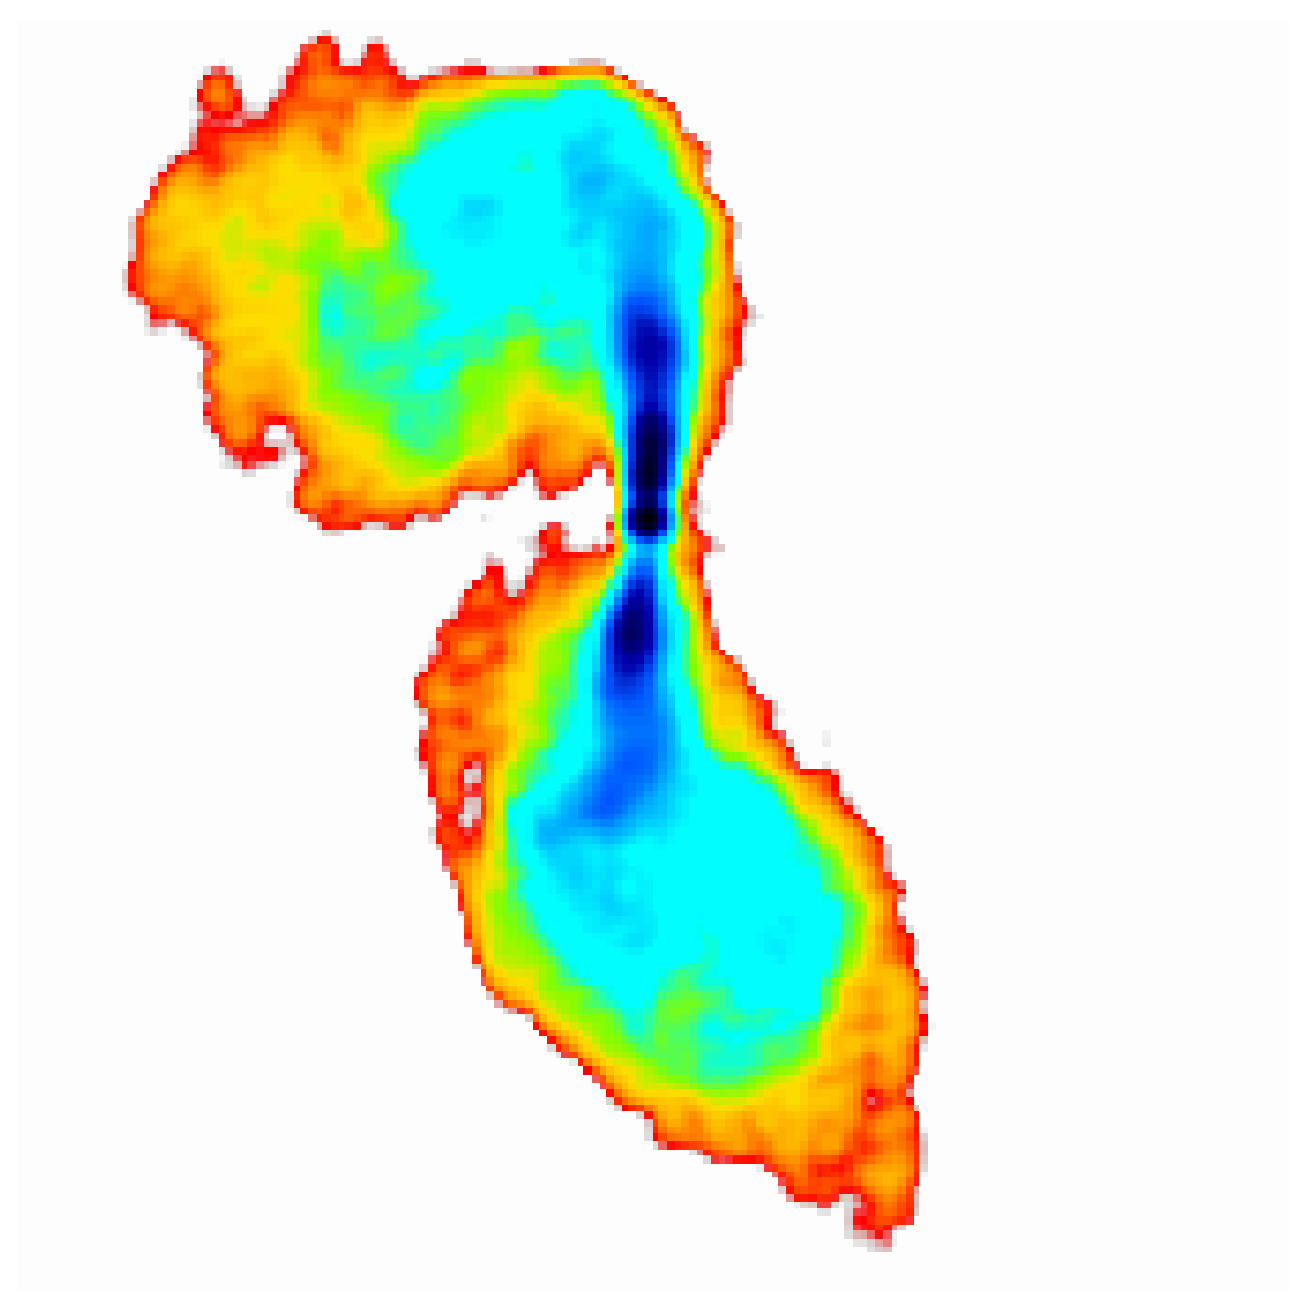
\includegraphics[width=\textwidth]{images/misc/3C272.1_FR_I_example}}
        \caption{ M84, an FR I jet}
    \end{subfigure}
    \begin{subfigure}[t]{0.635\textwidth}
        \frame{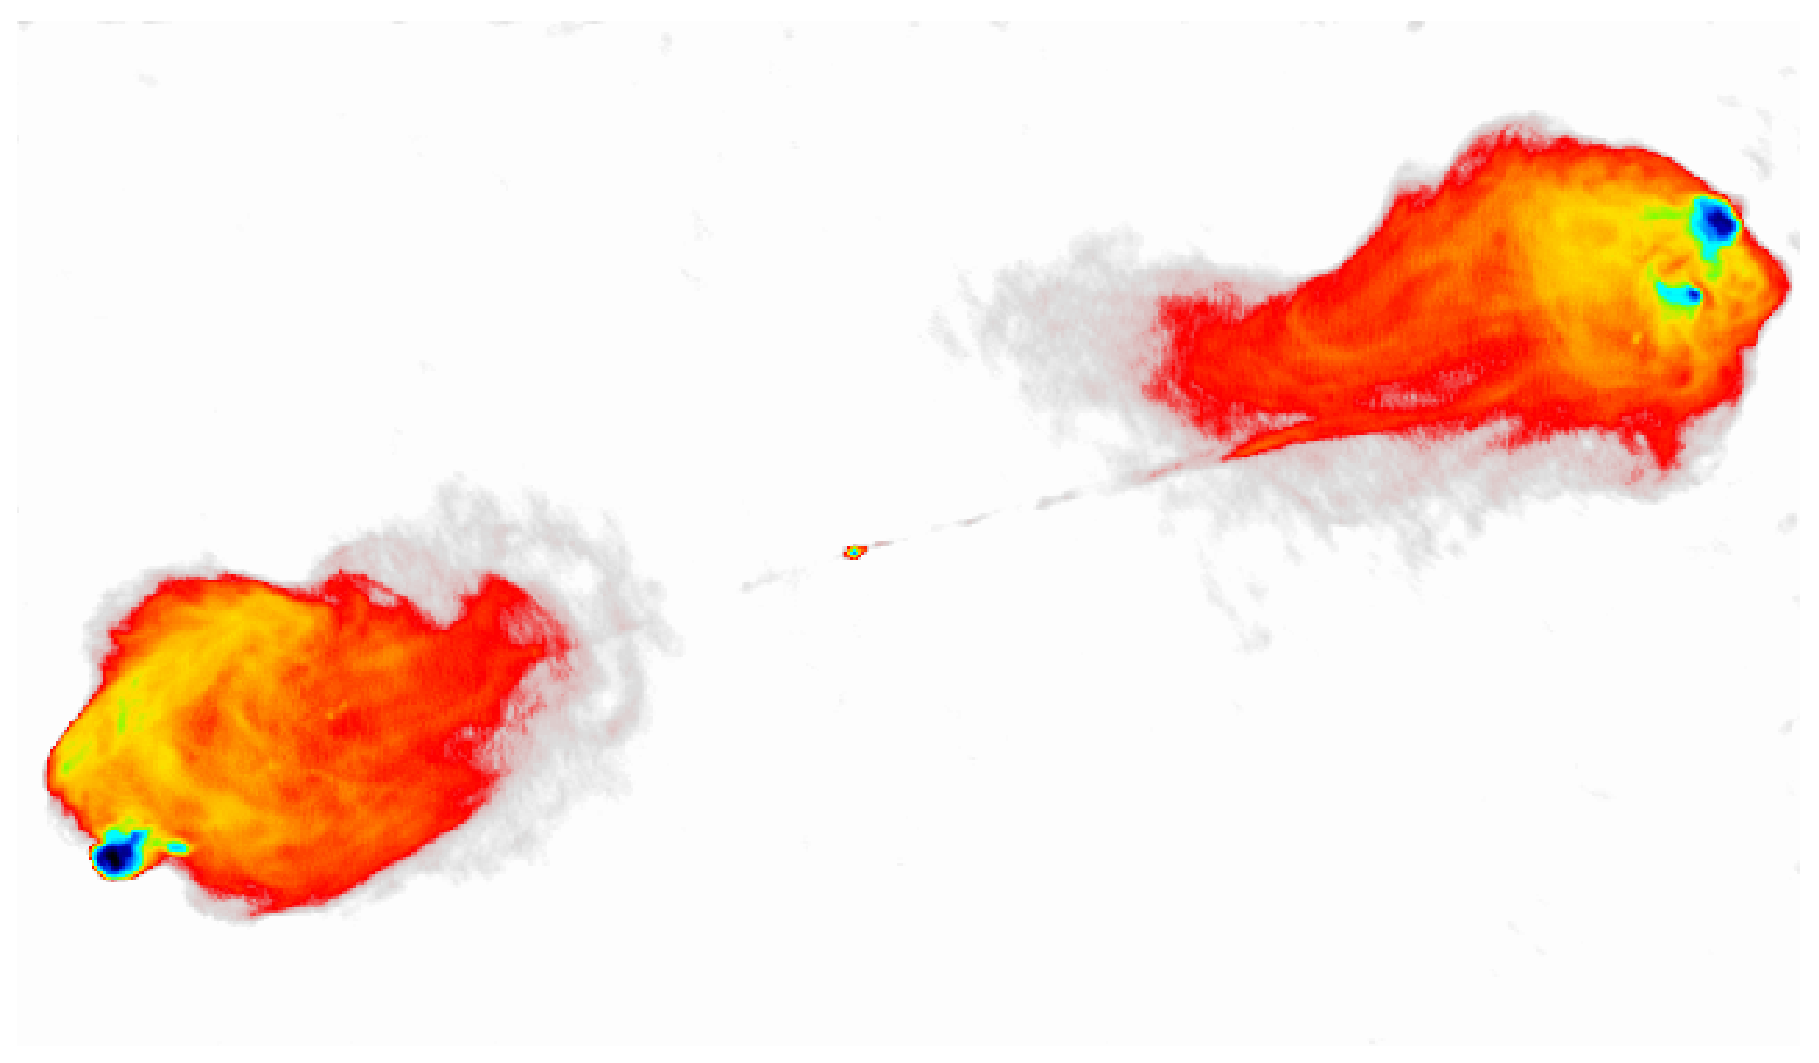
\includegraphics[width=\textwidth]{images/misc/CygA_FR_II_example}}
        \caption{Cygnus A, an FR II jet}
    \end{subfigure}
    %\frame{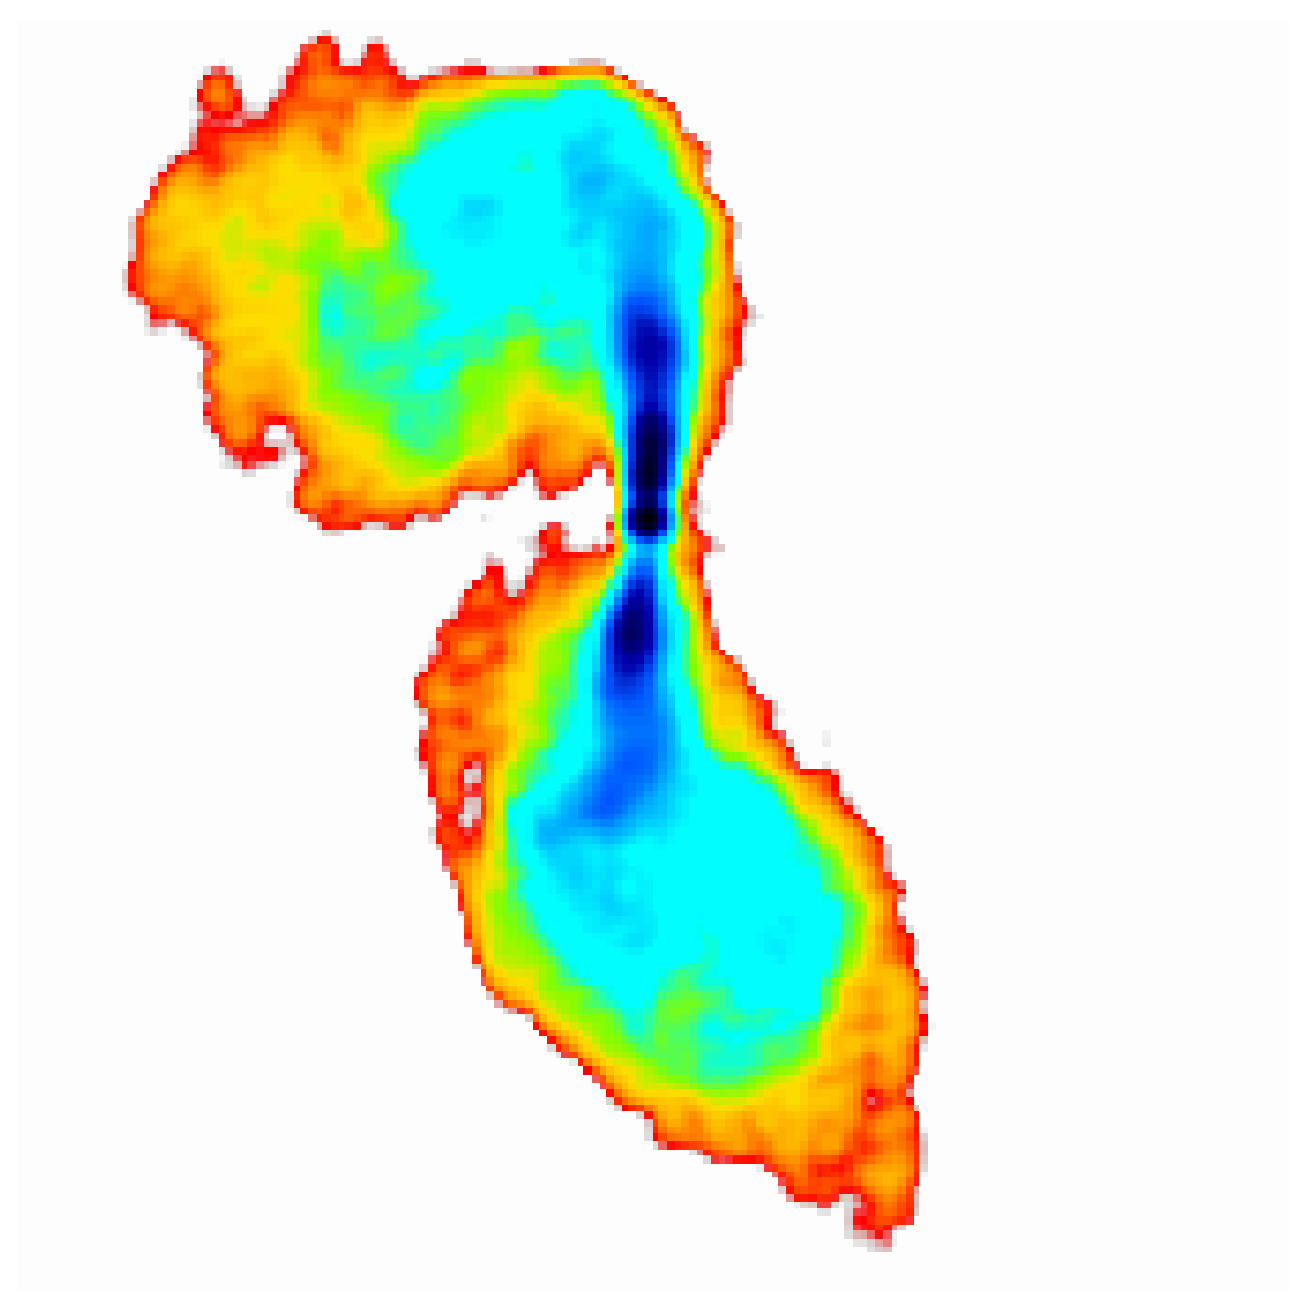
\includegraphics[width=0.365\textwidth]{images/misc/3C272.1_FR_I_example}}
    
    %\boxedfig{}{0.607\textwidth}{(b) FR II}
    %}
    \caption{Typical example images for the FR I and II classes. (a) shows an FR-I source, 3C272.1, image taken from DRAGN (http://www.jb.man.ac.uk/atlas/). The brightness of the jet gradually decreases away from the central nucleus (\textit{the core}). (b) shows an FR-II source, Cygnus A, taken from NED (http://ned.ipac.caltech.edu). Two bright hotspots and associated radio lobes lie on either side of the core that are connected by an otherwise invisible jet.\label{fig:FR_I_II} }
\end{figure}
\textit{Blazars} form another prominent class of jetted AGN in a sense the compliment to radio galaxies, as they are viewed with a small angle. They are further divided into two classes: flat-spectrum radio quasars (FSRQs), which display broad emission lines and BL Lacertae objects (BL Lacs), which have featureless spectra. Under the primary unification scheme 
\citep[e.g.,][]{urry1995unified}, FSRQs and BL Lacs are the closely aligned counterparts of FR-II type jets and FR-I type jets, respectively. Blazars have the highest apparent luminosity of all AGN families where the bulk relativistic motion causes enhancements in the apparent luminosity of up to $10^9$, a phenomenon known as \textit{relativistic beaming} (see section \ref{subsec:relativistic_effects}). The sources that are intermediate between radio galaxies and blazars are called Steep Spectrum Radio Quasars (SSRQs). The radio spectrum of the SSRQs is steeper than that of blazars, as there is a contribution from the lobe, which has a steeper spectrum, as opposed to the core, which has a flatter spectrum. Because of a major contribution from the beamed emission from the core, blazars appear as ``core dominated" while emission from the lobes constitute a major contributor to the observed emission in radio Galaxies, and hence they appear as ``lobe-dominated" \citep{1997iagn.book.....P}.
%Typically, the blazar category sources are observed to be ``core dominated"; the bulk of their radio emission comes from the relativistically beamed core. In contrast, the radio galaxies are observed to be ``lobe dominated"; the bulk of their radio emission comes from the lobes, which are not beamed. As the blazar jets are closely aligned, the beamed emission from their core overwhelms the emission from the lobe. Because the jets are aligned away from us in the radio galaxies, the emission from their lobes surpasses the de-beamed emission from their core.



\subsubsection{Non-jetted AGN}
These are the most common class of AGNs in the local universe, and Seyfert galaxies \citep{seyfert1943nuclear} are the first ones to be identified in this class. Typically, the Seyferts differ from other normal galaxies by their highly ionized emission lines and a bright, central core. Similar to the jetted AGNs, the Seyfert galaxies are divided into two classes based on their optical spectra \citep{khachikian1974atlas}: Seyfert I type, which display both narrow and broad emission lines, and Seyfert II type, which only display narrow emission lines (see Fig.~\ref{fig:agn_model}). Apart from the optical classification, the Sefyferts are also classified based on their X-ray emission, which relies on the intrinsic absorption in the soft X-ray band ($E\ll 5~\textrm{keV}$). A hydrogen absorption column density of $N_H=10^{22}~\textrm{cm}^{-2}$ draws the line between the type I and type II Seyferts. The ones above the threshold are strongly absorbed and fall into the type I class, while the ones below have lower absorption and fall into the type II class. 

There may also be sources with a low luminosity that go undetected in the all-sky surveys. For example, the bolometric luminosity of Sagittarius A*, which is the black hole at the center of our Milky Way galaxy, is less than $L_{bol}=10^{37}~\textrm{erg sec}^{-1}$. Such emission would not be detected if it were to lie in a distant galaxy. It is believed that these sources may have experienced some activity in the past and are presently undergoing a quiescent phase. Quasi Stellar Objects (QSO), or radio-quiet quasars are another type of non-jetted AGN. Note that, in the jet community, quasars refer to jetted-AGN with closely aligned jets, and unless otherwise stated a QSO refers to a non-jetted AGN. Similar to the Seyferts, the QSOs are further divided in to type I and type II, which display broad lines and only narrow lines, respectively. Unlike Seyferts, which often appear in spiral galaxies, the QSOs are generally seen in the elliptical ones.


